\documentclass[a4paper]{article}
\usepackage{graphicx, verbatim}
\usepackage[utf8]{inputenc}
%%\usepackage[czech]{babel}
\usepackage{amsmath,amssymb,amsthm,mathrsfs,amsfonts}
\usepackage{epigraph}

\usepackage{wasysym}
\setlength{\textwidth}{6.5in}
\setlength{\textheight}{9in}
\setlength{\oddsidemargin}{0in}
\setlength{\evensidemargin}{0in}
\setlength{\topmargin}{-1.5cm}
\renewcommand*{\theenumi}{\thesection.\arabic{enumi}}
\renewcommand*{\theenumii}{\theenumi.\arabic{enumii}}
\numberwithin{equation}{subsection}
\usepackage{Sweave}
\usepackage{hyperref}
\hypersetup{
    colorlinks=true, %set true if you want colored links
    linktoc=all,     %set to all if you want both sections and subsections linked
    linkcolor=blue,  %choose some color if you want links to stand out
}
\newtheorem*{tip}{Tip}

\title{MetaMass: tools for mass spectrometry data meta-analysis}
\author{Jan Stuchlý, Fridtjof Lund-Johansen}
\begin{document}

\maketitle
\begin{center}
{\tt jan.stuchly@lfmotol.cuni.cz}
\end{center}
%%chunk
\section{Introduction}
The presented package provides tools for meta-analysis of human proteome mass spectrometry (MS) data as described in (ref Lund-Johansen et al 2016). The purpose is to provide stand-alone tool for
analyzing text files or \texttt{data.frame} with an integration
with R for further analysis.
\\
Area of usage: MetaMass is a tool for meta-analysis of sub-cellular proteomics data (ref Lund-Johansen et al 2016). Users can analyze  mass spectrometry (MS) data  within the context of published datasets and sets of markers identified by mining of MS datasets or curated annotations from Uniprot, GO and the Human Protein Atlas. The input is text files with official human gene symbols as protein identifiers and normalized MS signal values measured in sub-cellular fractions. The output is a cdt file for visualization of the classified datasets as heatmaps in JavaTreeView, a table with with gene names, annotations, assigned locations and precision scores and precision-recall curves that provide information about the fit between the dataset and the marker set.

\noindent Required software:
\begin{itemize}
\item[] R (https://cran.r-project.org)
\item[] R Studio (https://www.rstudio.com) - for more user-friendly R-front-end
\item[] Rtools (https://cran.r-project.org/bin/windows/Rtools/)
  necessary on MS Windows operating system only
\item[] JavaTreeView (http://jtreeview.sourceforge.net/) - for visualisation
of heatmaps (the .cdt files - see below)
\end{itemize}
%% Installation:
%% Install devtools from R: \texttt{install.packages(``devtools'')}
%% load devtools: \texttt{library(devtools)}
%% Install MetaMass: \texttt{install_github(``stuchly/MetaMass'')}
%% load MetaMass: \texttt{library(MetaMass)}
%% see this vignette: \texttt{vignette("MetaMass")
\scriptsize
\begin{Schunk}
\begin{Sinput}
> install.packages("devtools") ##  Install devtools from R
> library(devtools) ## load devtools
> install_github("stuchly/MetaMass") ## Install MetaMass
> library(MetaMass) ## load MetaMass
> vignette("MetaMass") ## see this vignette
\end{Sinput}
\end{Schunk}
\normalsize
\section{Input}
 On input user provides a
\texttt{data.frame} containing the MS data or path to text file(s)
with the data. Data are
then processed with respect to following conventions:
\begin{itemize}
  \item All columns containing numerical values only are used as MS data
    \item MS data could be divided into different groups'' if separated
      by blank/non-numeric column i.e. numeric columns flanked by
      non-numeric columns are understood as a single "group''.
      With more file on input each file is considered as separate set
      of groups.
    \item \texttt{data.frame} must contain a column containing protein
      ID which match the annotation file (by default the genename in
      the first column;see below)
      \item by default tab-delimited text file is assumed
      \item trailing spaces in character columns are removed
  \end{itemize}
  An annotation file is provided in the package
 \scriptsize
\begin{Schunk}
\begin{Sinput}
> library(MetaMass)
> data(AnnotationAM)
> head(AnnotationAM)
\end{Sinput}
\begin{Soutput}
  Uniprot   Gene Christoforou_Uniprot_G.O_overlap Christoforou_Uniprot_G.O_sum
1  P04217   A1BG                                                              
2  Q9NQ94   A1CF                                                              
3  P01023    A2M                                                              
4  A8K2U0  A2ML1                                                              
5  Q9NPC4 A4GALT                            Golgi                        Golgi
6  Q9UNA3  A4GNT                            Golgi                        Golgi
  HPA_Single_supportive HPA_Single_uncertain HPA_main_supportive
1                                                               
2               Nucleus                                  Nucleus
3                                                               
4                                                               
5                                                               
6                                                               
  HPA_main_uncertain ChristoforouUniprot_G.Ooverlap_CMN
1                                                      
2                                                      
3                                                      
4                                                      
5                                              membrane
6                                              membrane
\end{Soutput}
\end{Schunk}
\normalsize
\subsection{Troubleshooting}
The common challenge for new users of R is data import. The function
\texttt{analyze.MSfile} expects tab-delimited file which could be
read via function \texttt{read.table()}
\scriptsize
\begin{Schunk}
\begin{Sinput}
> data_table<-read.table(filename,header=TRUE,sep="\t")
\end{Sinput}
\end{Schunk}
\normalsize
If there is an error concerning reading the input file, the user can
try this function to check if the file is in correct format.
The other possible issue is the grouping of the data columns. As
mentioned above each contiguous sequence of numerical columns
(flanked by non-numeric column) is considered as one group - the user
can check if all (and only) the data he wants to analyze would be
considered as MS data as follows
\scriptsize
\begin{Schunk}
\begin{Sinput}
> colnames(data_table)[sapply(data.table,is.numeric)]
\end{Sinput}
\end{Schunk}
\normalsize
\subsection{Custom Annotation file}
By default the marker sets in data.frame \texttt{AnnotationAM} are
used however the user can provide a custom Annotation file which meets
the following conventions

\begin{itemize}
  \item the file is tab-delimited (by default)
  \item the first column contains the Uniprot IDs
    \item the localisations identifiers must be empty string or syntactically valid
      names (i.e. a string which consists of letters, numbers, and the dot and (for versions of R at least 1.9.0) underscore characters, and starts with either a letter or a dot not followed by a number. Reserved words are not syntactic names)
  \end{itemize}
  The localisations will be sorted in the following order
  \scriptsize
\begin{Schunk}
\begin{Sinput}
> data(levelsC)
> levelsC
\end{Sinput}
\begin{Soutput}
 [1] "CYTOSOL"              "CS"                   "RIBOSOME"            
 [4] "ENDOSOME"             "LYSOSOME"             "PM"                  
 [7] "MEMBRANE"             "ER"                   "GOLGI"               
[10] "MITOCHONDRION"        "NUCLEUS"              "EXTRACELLULAR_MATRIX"
\end{Soutput}
\end{Schunk}
\normalsize
and the localisations not present in \texttt{levelsC} will be sorted
  in lexicographical order after those present in \texttt{levelsC}.
\section{Output}
By default (with parameter \texttt{output=NULL}) the user level function
\texttt{analyze.MSfile} does not create any files in the working
directory and returns named list to be analyzed within R (see
below). However most of the users are expected to specify the
parameter \texttt{output=\char`\"name\char`\"} and inspect the results outside
R. In this case three files will be created in the working directory.
\begin{itemize}
  \item name\_table.txt - spreadsheet containing the analyzed data and
    all annotations used (see below) for the analysis together the
    cluster assignment and precision with respect to the most abundant component
    \item name\_pr.pdf - precision-recall curves of the
      cluster assignment with respect to all used annotations
       \item name\_pr\_abs.pdf - number of assigned proteins versus the
         precision of clusters with respect given localization
      \item name\_javatree.cdt - heatmap to be visualized in the Java
        TreeView application. Each line is annotated by the protein
        ID, annotation (Annot=;if present for this protein) and
        assignment (assign=;assignment of the cluster containing
        this protein)
  \end{itemize}
\section{Metadata}
The package is distributed with MS data which could be used to
reproduce the results in the paper or as a reference for user supplied
data - these data are called Metadata - see \texttt{?Metadata.}
The Metadata can be used as \texttt{data.frame} or if the user want to
open then in a spreadsheet editor their location on the computer can
be found via \texttt{system.file} function.
\scriptsize
\begin{Schunk}
\begin{Sinput}
> filename<-system.file("extdata","Bileck.txt",package="MetaMass")
> filename
\end{Sinput}
\begin{Soutput}
[1] "/Library/Frameworks/R.framework/Versions/3.2/Resources/library/MetaMass/extdata/Bileck.txt"
\end{Soutput}
\end{Schunk}
\normalsize
\section{Walk-through}
In this section we give detailed description how create and analyze
the MS data files. This section is intended for users with minimal
experience with R. If the reader wants to avoid downloading a creating
this files he can find the same examples in the section \hyperref[examp_s]{Examples} where the same internally stored datasets are used.
See \texttt{?analyze.MSfile} for detailed information.
\\
Preparation of datasets and marker set for testing of the tool.

1. Copy contents of supplementary table 1.13 (Data Fig2a)  into new spreadsheet. Delete columns B:L (Christoforou data) . Save as tab-delimited text in folder named e.g. Test, name the file Data\_Fig.2a
2. Copy contents of supplementary table 1.14 (study4\_9\_10)  into new spreadsheet. Save as tab-delimited text in folder named e.g. Test, name the file study4\_9\_10.txt
3. Copy contents in supplementary Table 1.11, (Annotation Table R-version) . Copy data into new spreadsheet.  Save as tab-delimited text in folder named e.g. Test, name the file MyMarkers

\subsection{Analysis option 1}
\label{opt1}
see \hyperref[ex2]{Example 2}
Generate the heatmap and the classification output files corresponding to Fig. 2a in the article:
(typed commands are in script font, those below can be copied and pasted into R-studio, complete commands by pressing the enter key.)
\scriptsize
\begin{Schunk}
\begin{Sinput}
> library(MetaMass)
> analyze.MSfile(MSfile = "Data_Fig2a.txt",Metadata = "Christoforou",overlap = 2, clusters = 1400, Annotation = "MyMarkers.txt", markers =c(3,4,7), output = "Fig2a")
\end{Sinput}
\end{Schunk}
\normalsize
\begin{tip}
Typing in R-Studio is greatly simplified using the tab key to
auto-complete the command.. Thus, the command above can be typed as
follows:  ana [tab], msf [tab], “dat [tab], meta [tab],
“Christoforou”), out [tab], “Fig1b”)
\end{tip}
Explanation: analyze.MSfile: name of function used to perform all the analyses.
MSfile: dataset to be analyzed,
Metadata (see \texttt{?Metadata}): The “Christoforou” dataset is one of several stored in MetaMass as reference data. A complete list is found in supplementary Table 1.10.  The meta-data is not clustered or used for the classification, but simply aligned to the processed test dataset as reference. Overlap=2 . The analysis is restricted to proteins that are identified both in the dataset and the metadata.
Clusters: number of clusters to generate in K-means clustering. (an average cluster size of 5 is recommended)
Annotation: Text file with marker lists, number corresponds to column number in the file. Markers: c(3,4,7) use marker sets in columns 3,4, and 7 in the annotation list.
output: file-prefix for the output files.
\\
Result: The output files are found in the working directory. All output files have the prefix “Fig2a”.
Fig2a.cdt file is a heatmap  file (JavaTreeView), The algoritm generates a single heatmap corresponding to the first of the marker sets, in this case marker set 3. (Uniprot/GO overlap + study 1).
Fig.2a\_table.txt is the classification result table (open with e.g Excel). The table contains protein identifiers, annotations from HPA, Uniprot and GO, the location assigned by MetaMass and the precision. The table also contains the MS signal values.
Fig2a\_pr-pdf contains precision-recall curves with relative numbers on the y-axis(e.g. Acrobat Reader).
Fig2a\_pr\_abs.pdf contain precision recall curves with absolute numbers on the y-axis. These numbers correspond to the number of mapped proteins.

\subsection{Analysis option 2}
\label{opt2}
See \hyperref[ex4]{Example 4}
Compare results obtained when datasets 4, 9 and 10 are analyzed, and
study 1 is used as metadata, and vice versa.  (supplementary
Fig. 14). Analyze dataset1, use dataset 4,9 and10, as Metadata.
\scriptsize
\begin{Schunk}
\begin{Sinput}
> analyze.MSfile(MSfile = "study1.txt", clusters=432, Metadata = c("Carvalho", "Bileck", "Thakar"), Annotation = "MyMarkers.txt", markers=c(3,4,6,7,9), output = "study1_MyMark")
\end{Sinput}
\end{Schunk}
\normalsize
Analyze dataset 4,9 and 10, use dataset1 as Metadata
\scriptsize
\begin{Schunk}
\begin{Sinput}
> analyze.MSfile(MSfile = "study4_9_10.txt",clusters = 473,Annotation = "MyMarkers.txt", markers=c(3,4,6,7,9),output = "study4_9_10_MyMark")
\end{Sinput}
\end{Schunk}
\normalsize

The heatmaps are shown in supplementary Fig. 14. The pie chart in the figure shows the frequency of proteins that were mapped to the same location, different locations, not mapped, and those that were mapped using one of the datasets only. Even though studies 4 9 and 11 used low resolution methods, 80\% of proteins that were mapped to a location in both analyses are mapped to the same locations as in study 1 when the data are combined.
\subsection{Analysis option 3}
\label{opt3}
See \hyperref[ex7]{Example 7}
Compare heatmaps obtained when the data in Fig. 2a are analyzed using a wide range of marker sets from Uniprot, GO and the Human Protein Atlas  (supplementary Fig. 16)
\scriptsize
\begin{Schunk}
\begin{Sinput}
> analyze.MSfile(MSfile = "Data_Fig2a.txt", Annotation = "MyMarkers.txt", markers=9, clusters=1400, output = "Fig2aSVM")
> analyze.MSfile(MSfile = "Data_Fig2a.txt", Annotation = "MyMarkers.txt", markers=4, clusters=1400, output = "Fig2aUGOovl")
> analyze.MSfile(MSfile = "Data_Fig2a.txt", Annotation = "MyMarkers.txt", markers=3, clusters=1400, output = "Fig2aStudy1UGOovl")
> analyze.MSfile(MSfile = "Data_Fig2a.txt", Annotation = "MyMarkers.txt", markers=6, clusters=1400, output = "Fig2aUniGOsum")
> analyze.MSfile(MSfile = "Data_Fig2a.txt", Annotation = "MyMarkers.txt", markers=7, clusters=1400, output = "Fig2aHPAsupportive")
> analyze.MSfile(MSfile = "Data_Fig2a.txt", Annotation = "MyMarkers.txt", markers=8, clusters=1400, output = "Fig2aHPAuncertain")
\end{Sinput}
\end{Schunk}
\normalsize
%% \subsection{Analysis option 4}
%% \label{opt4}
%% Generate recall-precision curves for single datasets (i.e. similar to Fig. 2b in article)
%% \scriptsize
%% @
%% <<eval=false>>=
%% analyze.MSfile(MSfile = "study4.txt", Metadata = "Christoforou", output = "study4")
%% @ %def
%% \normalsize
%% Result: The recall response curves for cytosol and nucleus are similar to those for study 4 in Fig2a.
%% \subsection{Analysis option 5}
%% \label{opt5}
%% see \hyperref[ex3]{Example 3}
%% Perform a meta-analysis of datasets 4, 9 and 10.
%% \scriptsize
%% @
%% <<eval=false>>=
%% analyze.MSfile(MSfile = c("study4.txt","study9.txt", "study10.txt"), Metadata = "Christoforou", output = "study4910")
%% @ %def
%% \normalsize
%% Explanation: c("study4.txt","study9.txt", "study10.txt") is used to merge data from multiple files into one analysis. The file contains the overlap of these three and the Christoforou dataset used as metadata.
%% \\
%% Result: The fractionation methods used in studies 4, 9 and 10 have
%% limited resolution. However, combined they have high resolution. Thus,
%% study 4 has high resolution of mitochondria, but poor separation of ER
%% and nuclei. Study 9 has good separation of cytoplasmic organelles and
%% nuclei, but no resolution of ER, mitochondria or cytosol. Study 9 has
%% good resolution of cytosol, membranes and nuclei, but does not
%% discriminate ER from mitochondria. When the datasets are combined,
%% they complement each other. See figure \ref{opt5}

%% \begin{figure}[b]
%% 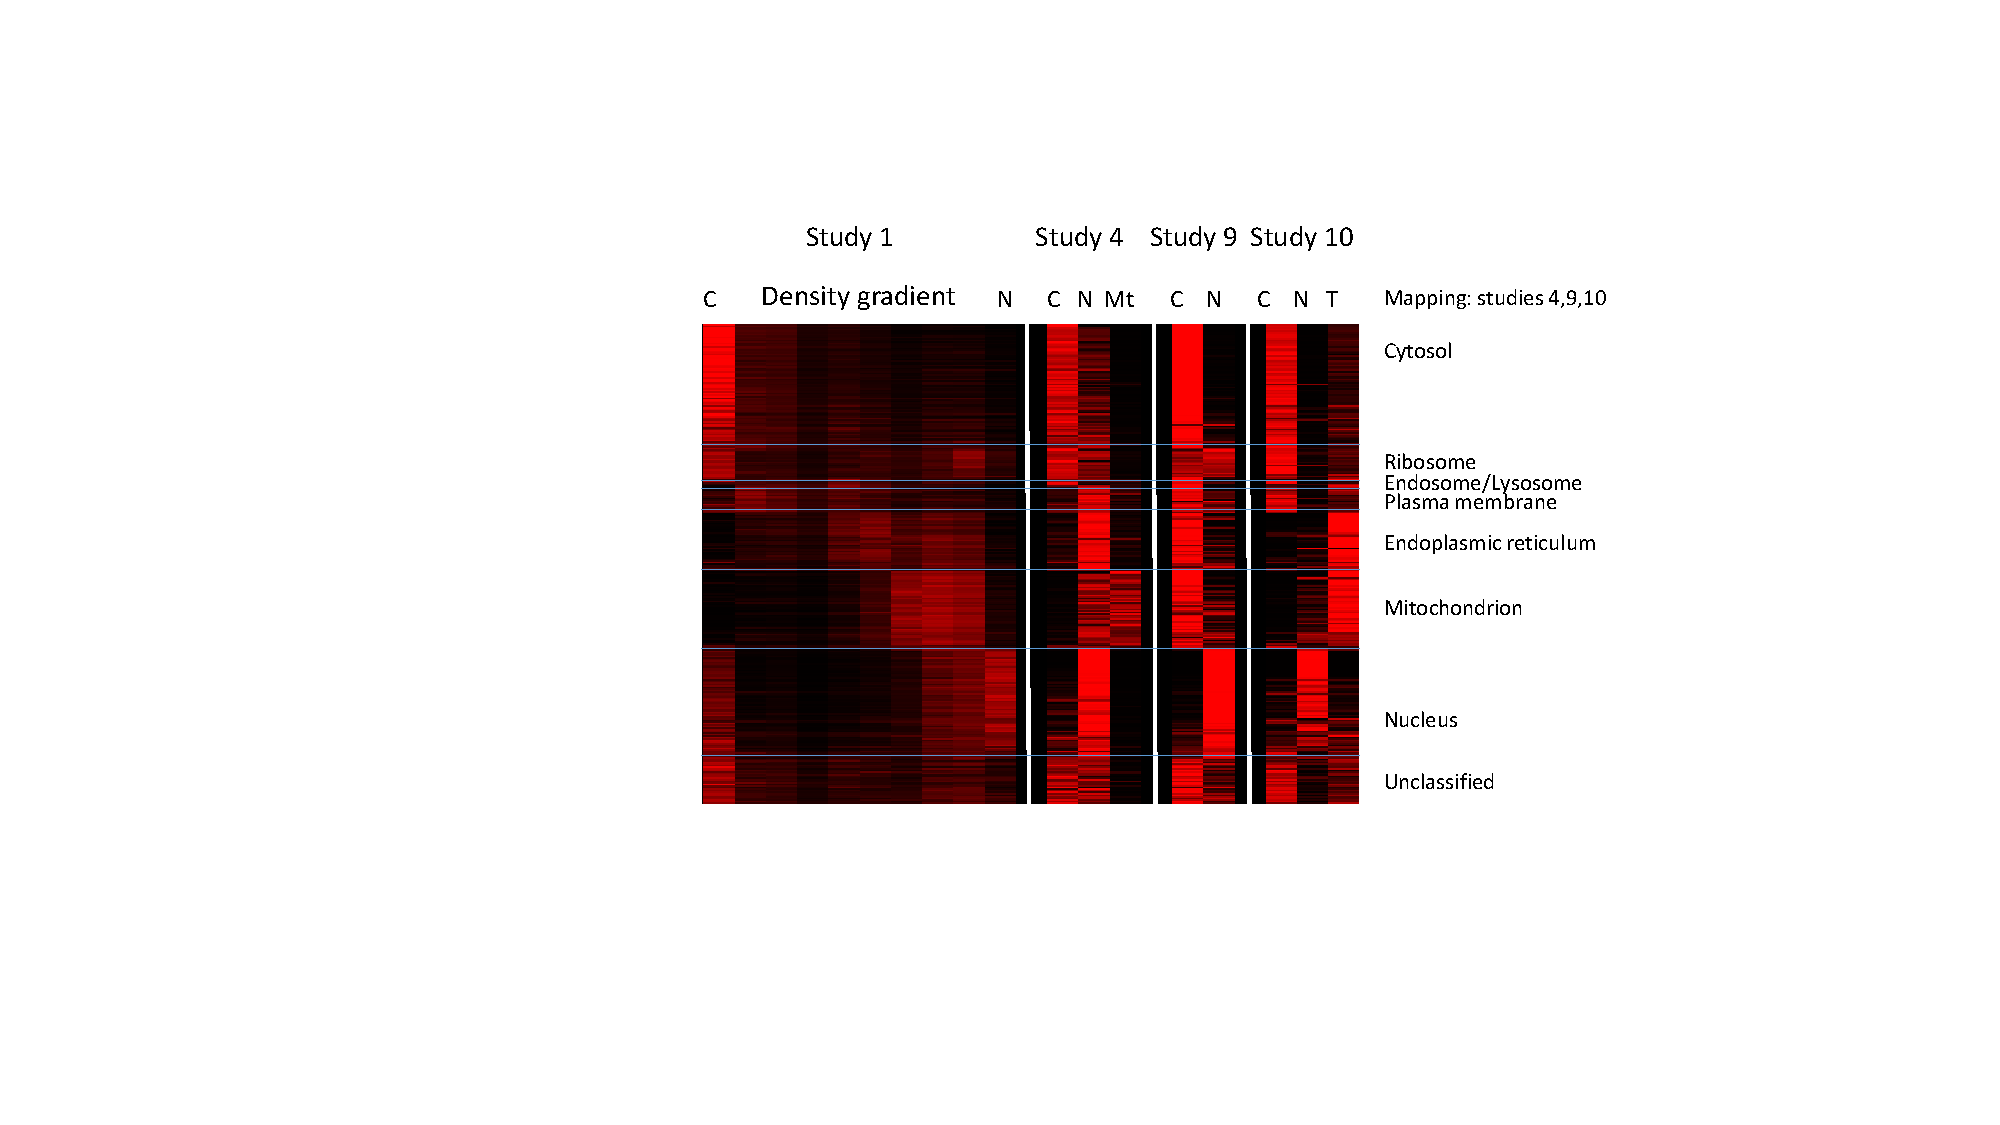
\includegraphics{opt5.pdf}
%% \caption{Heatmnap as seen in JavaTreeView}
%% \label{opt5}
%% \end{figure}
\subsection{Additional user-selectable variables}
Number of groups in K-means clustering : The default option is 500 groups. The optimal number of proteins per group is 10-20. If the dataset has more than 5000 proteins or less than 3000 proteins users may specify the number of groups accordingly.  The command clusters= 250 specifies 250 clusters.
Comparison metrics: The default option is Euclidean distance. The
command… metric =”correlation” specifies Pearson correlation (see \texttt{?analyze.MSfile}).
\section{Analysis within R}
Although the main purpose of this package is to create annotated lookup
tables and heatmaps which can be conveniently analyzed outside R the
results can be naturally treated as any R object.
The function \texttt{analyze.MSfile} returns named list containing the
original data, annotation(s) and cluster assignments. Two function
can be used to extract it's contents - see \texttt{?get.data} and \texttt{?get.clusters}.
\scriptsize
\begin{Schunk}
\begin{Sinput}
> file2<-system.file("extdata","Data_Fig_1b.txt",package="MetaMass")
> ##cluster with respect MSfile only (cluster.metadata=FALSE by default)
> res2<-analyze.MSfile(MSfile=file2,Metadata=c("Christoforou"),output="res2",markers=c(3:5))
> data2<-get.data(res2,data.only=TRUE)
> cls2_1<-get.clusters(res2,rID=1) #rID=1 annotation with respect to markers[1]; default
> head(cls2_1)
\end{Sinput}
\begin{Soutput}
  cluster GOLGI CYTOSOL ER MITOCHONDRION NUCLEUS PM LYSOSOME PEROXISOME CS
1       1     0       0  0             0       0  1        0          0  0
2       2     0       0  2             0       1  0        0          0  0
3       3     0       0  0             0       2  0        0          0  0
4       4     0       1  0             0       0  0        0          0  1
5       5     0       0  3             1       0  0        1          0  0
6       6     0       1  0             0       0  0        0          0  0
  ENDOSOME EXTRACELLULAR RIBOSOME Nb_of_annotations precision_main_component
1        0             0        0                 1                1.0000000
2        0             0        0                 3                0.6666667
3        0             0        0                 2                1.0000000
4        0             0        0                 2                0.5000000
5        2             1        0                 8                0.3750000
6        0             0        0                 1                1.0000000
  main_component GOLGI_ratio CYTOSOL_ratio  ER_ratio MITOCHONDRION_ratio
1             PM           0           0.0 0.0000000               0.000
2             ER           0           0.0 0.6666667               0.000
3        NUCLEUS           0           0.0 0.0000000               0.000
4        CYTOSOL           0           0.5 0.0000000               0.000
5             ER           0           0.0 0.3750000               0.125
6        CYTOSOL           0           1.0 0.0000000               0.000
  NUCLEUS_ratio PM_ratio LYSOSOME_ratio PEROXISOME_ratio CS_ratio
1     0.0000000        1          0.000                0      0.0
2     0.3333333        0          0.000                0      0.0
3     1.0000000        0          0.000                0      0.0
4     0.0000000        0          0.000                0      0.5
5     0.0000000        0          0.125                0      0.0
6     0.0000000        0          0.000                0      0.0
  ENDOSOME_ratio EXTRACELLULAR_ratio RIBOSOME_ratio assigned_location
1           0.00               0.000              0                PM
2           0.00               0.000              0                ER
3           0.00               0.000              0           NUCLEUS
4           0.00               0.000              0                CS
5           0.25               0.125              0                ER
6           0.00               0.000              0           CYTOSOL
  Nb_main_component Nb_assigned_location precision_assigned_location
1                 1                    1                   1.0000000
2                 2                    2                   0.6666667
3                 2                    2                   1.0000000
4                 1                    2                   1.0000000
5                 3                    3                   0.3750000
6                 1                    1                   1.0000000
  updated_order
1           189
2           256
3           444
4           105
5           253
6            71
\end{Soutput}
\end{Schunk}
\normalsize
Here we have extracted the data accompanied only by the protein ID and
the cluster ID together with the analysis results with respect to the
first marker set.
As the the clusters in the \texttt{cls2\_1} \texttt{data.frame} are
ordered by the cluster ID we can add any information to the data e.g.
\scriptsize
\begin{Schunk}
\begin{Sinput}
> data2<-data.frame(data2,main_component1=cls2_1$main_component[data2$cluster])
\end{Sinput}
\end{Schunk}
\normalsize
\section{Examples}
\label{examp_s}
The simplest way to use this package is the wrapper function
\texttt{analyze.MSfile} (see \texttt{?analyze.MSfile}). This function
reads and process your the tab-delimited text file with MS data and
stores the results in the working directory.
Set working directory: In R-studio go to menu: Session, select set working directory, identify the folder where your data are stored. The output files will also appear in this folder.
After setting the working directory, it is necessary to provide the
path to the tab-delimited file with MSdata. As the first example we use the data from figure 2a in the paper without the first
(reference;metadata) columns.
\subsection{Example 1}
\label{ex1}
\scriptsize
\begin{Schunk}
\begin{Sinput}
> file1<-system.file("extdata","Data_Fig_1a.txt",package="MetaMass")
\end{Sinput}
\end{Schunk}
\normalsize
The function MetaMass recognizes two types of data -
\texttt{MSfile} and \texttt{Metadata}. The \texttt{MSfile} are the
actual data to be analyzed whereas the Metadata stand for internally
stored MSdata which can be used as reference (see
\texttt{?Metadata}).
\scriptsize
\begin{Schunk}
\begin{Sinput}
> ##proteins identified by gene-name -> annotation.ID=2 (see ?AnnotationAM)
> ##cluster with respect metadata only (group=0)
> res1<-analyze.MSfile(MSfile=file1,Metadata=c("Christoforou"),output="res1",group=0,cluster.metadata=TRUE)
\end{Sinput}
\end{Schunk}
\normalsize
In this case (compare the command to the \texttt{usage} section in
\texttt{?analyze.MSfile}) we use the default annotation, as Metadata
we use the  Christoforou, Mulvey, Breckels, et al. (2016) dataset and the
output will be stored in files starting with the string 'res1'. As a
toy example (to get the similar result as in figure 1a) we want to
cluster only the metadata and align the \texttt{MSfile} - do this we
set \texttt{group=0} which says that none of the data in MSfile should
be clustered and we have to specify that want cluster the metadata \texttt{cluster.metadata=TRUE}).
\\
\subsection{Example 2}
\label{ex2}
As the second example let us reconstruct the figure 2a in the
paper. Here we want to cluster the MSfile (which is default and we
need not specify the \texttt{group} parameter) and align the metadata
to it.
\scriptsize
\begin{Schunk}
\begin{Sinput}
> file2<-system.file("extdata","Data_Fig2a.txt",package="MetaMass")
> MyMarkers<-system.file("extdata","MyMarkers.txt",package="MetaMass")
> ##cluster with respect MSfile only (cluster.metadata=FALSE by default)
> library(MetaMass)
> analyze.MSfile(MSfile = file2,Metadata = "Christoforou",overlap = 2, clusters = 1400, Annotation = MyMarkers, markers =c(3,4,7), output = "Fig2a")